\documentclass[aspectratio=169,10pt]{beamer}
\usetheme{Madrid}
\usecolortheme{default}

\usepackage{amsmath}
\usepackage{amssymb}
\usepackage{booktabs}
\usepackage{graphicx}
\usepackage{tikz}
\usetikzlibrary{arrows,positioning,shapes,backgrounds,fit}
\usepackage{pgfplots}
\pgfplotsset{compat=1.18}

% Custom colors
\definecolor{darkblue}{RGB}{0,51,102}
\definecolor{lightblue}{RGB}{51,153,255}
\definecolor{darkgreen}{RGB}{0,102,51}
\definecolor{orange}{RGB}{255,128,0}
\definecolor{darkred}{RGB}{153,0,0}

\setbeamercolor{structure}{fg=darkblue}
\setbeamercolor{frametitle}{bg=darkblue,fg=white}

\title{LOM: A Large Optimization Model for near-real time large-scale power system flexibility scenario exploration}
\author{Théotime Coudray}
\institute{UVSQ - PowDev}
\date{\today}

\begin{document}

% Title slide
\begin{frame}
\titlepage
\end{frame}

% Outline
\begin{frame}{Outline}
\tableofcontents
\end{frame}

\section{Problem Motivation}

\begin{frame}{The Unit Commitment Challenge}
\begin{columns}
\column{0.5\textwidth}
\textbf{What is Unit Commitment?}
\begin{itemize}
    \item Optimize power system operations over 24h, at 15 min time resolution
    \item Decide which generators to turn on/off
    \item Schedule generation to meet demand
    \item Minimize total system cost
\end{itemize}

\vspace{1em}
\textbf{Why is it Hard?}
\begin{itemize}
    \item Mixed-Integer Linear Program (MILP)
    \item NP-hard combinatorial problem
    \item Large-scale: 100+ zones, 96 timesteps
    \item Hours to solve with commercial solvers
\end{itemize}

\column{0.5\textwidth}
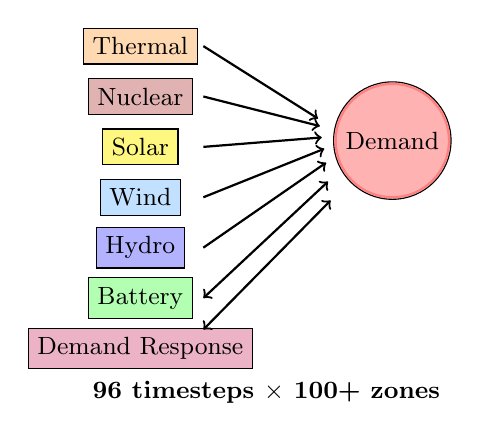
\begin{tikzpicture}[scale=0.8]
    % Generators
    \node[draw,rectangle,fill=orange!30] at (0,3) {\small Thermal};
    \node[draw,rectangle,fill=darkred!30] at (0,2.2) {\small Nuclear};
    \node[draw,rectangle,fill=yellow!50] at (0,1.4) {\small Solar};
    \node[draw,rectangle,fill=lightblue!30] at (0,0.6) {\small Wind};
    \node[draw,rectangle,fill=blue!30] at (0,-0.2) {\small Hydro};
    \node[draw,rectangle,fill=green!30] at (0,-1.0) {\small Battery};
    \node[draw,rectangle,fill=purple!30] at (0,-1.8) {\small Demand Response};
    
    % Demand with surrounding circle
    \node[draw,circle,fill=red!30,minimum size=0.8cm] (demand_inner) at (4,1.5) {\small Demand};
    \draw[thick,red!50] (4,1.5) circle (0.9cm);
    
    % Connections - arrows point to outer circle
    \draw[->,thick] (1,3) -- (2.82,1.85);
    \draw[->,thick] (1,2.2) -- (2.85,1.73);
    \draw[->,thick] (1,1.4) -- (2.88,1.55);
    \draw[->,thick] (1,0.6) -- (2.92,1.37);
    \draw[->,thick] (1,-0.2) -- (2.95,1.15);
    \draw[<->,thick] (1,-1.0) -- (2.98,0.85);
    \draw[<->,thick] (1,-1.5) -- (3.02,0.55);
    
    \node at (2,-2.5) {\small \textbf{96 timesteps $\times$ 100+ zones}};
\end{tikzpicture}
\end{columns}
\end{frame}

\begin{frame}{Asset-Level Complexity}
\begin{center}
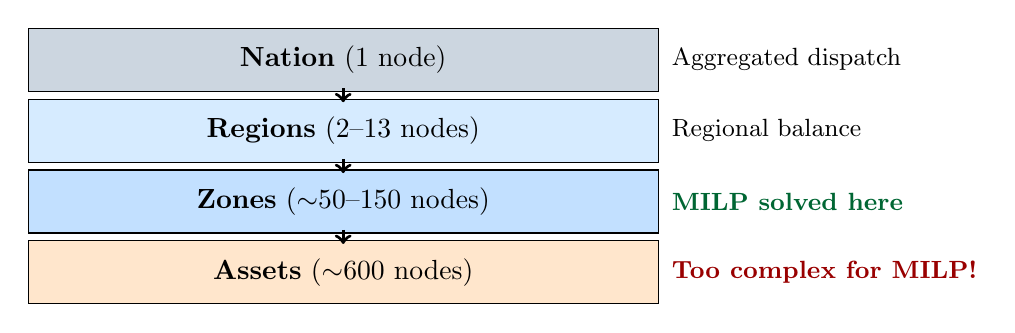
\begin{tikzpicture}[scale=0.9]
    % Hierarchy
    \node[draw,rectangle,fill=darkblue!20,minimum width=8cm,minimum height=0.8cm] at (0,3) {\textbf{Nation} (1 node)};
    \node[draw,rectangle,fill=lightblue!20,minimum width=8cm,minimum height=0.8cm] at (0,2) {\textbf{Regions} (2--13 nodes)};
    \node[draw,rectangle,fill=lightblue!30,minimum width=8cm,minimum height=0.8cm] at (0,1) {\textbf{Zones} ($\sim$50--150 nodes)};
    \node[draw,rectangle,fill=orange!20,minimum width=8cm,minimum height=0.8cm] at (0,0) {\textbf{Assets} ($\sim$600 nodes)};
    
    % Arrows
    \draw[->,very thick] (0,2.6) -- (0,2.4);
    \draw[->,very thick] (0,1.6) -- (0,1.4);
    \draw[->,very thick] (0,0.6) -- (0,0.4);
    
    % Annotations
    \node[align=left,anchor=west] at (4.5,3) {\small Aggregated dispatch};
    \node[align=left,anchor=west] at (4.5,2) {\small Regional balance};
    \node[align=left,anchor=west] at (4.5,1) {\small \textcolor{darkgreen}{\textbf{MILP solved here}}};
    \node[align=left,anchor=west] at (4.5,0) {\small \textcolor{darkred}{\textbf{Too complex for MILP!}}};
\end{tikzpicture}
\end{center}

\vspace{1em}
\textbf{Complexity Explosion at Asset Level:}
\begin{itemize}
    \item \textcolor{darkred}{$>$1M continuous variables, $>$50K binary variables}
    \item \textcolor{darkred}{$>$1.4M constraints}
    \item \textcolor{darkred}{Solve time: days instead of minutes}
\end{itemize}
\end{frame}

\section{Project Architecture}

\begin{frame}{End-to-End Pipeline}
\begin{center}
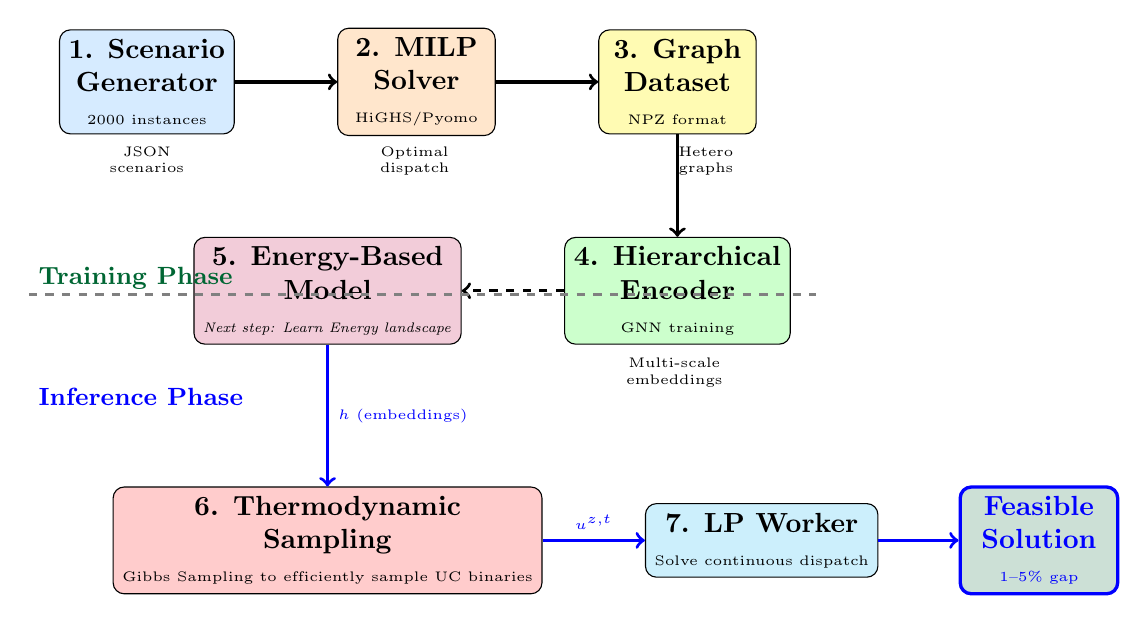
\begin{tikzpicture}[node distance=1.3cm,
    box/.style={rectangle,draw,rounded corners,align=center,minimum width=2.0cm,minimum height=0.9cm}]
    
    % Training phase (top)
    \node[box,fill=lightblue!20] (gen) {\textbf{1. Scenario}\\\textbf{Generator}\\{\tiny 2000 instances}};
    \node[box,fill=orange!20,right=of gen] (milp) {\textbf{2. MILP}\\\textbf{Solver}\\{\tiny HiGHS/Pyomo}};
    \node[box,fill=yellow!30,right=of milp] (graph) {\textbf{3. Graph}\\\textbf{Dataset}\\{\tiny NPZ format}};
    \node[box,fill=green!20,below=of graph] (encoder) {\textbf{4. Hierarchical}\\\textbf{Encoder}\\{\tiny GNN training}};
    \node[box,fill=purple!20,left=of encoder] (ebm) {\textbf{5. Energy-Based}\\\textbf{Model}\\{\tiny \textit{Next step: Learn Energy landscape}}};
    
    % Inference phase (bottom) - NEW
    \node[box,fill=red!20,below=of ebm,yshift=-0.5cm] (thermo) {\textbf{6. Thermodynamic}\\\textbf{Sampling}\\{\tiny Gibbs Sampling to efficiently sample UC binaries}};
    \node[box,fill=cyan!20,right=of thermo] (lp) {\textbf{7. LP Worker}\\\tiny{Solve continuous dispatch}};
    
    % Training flow arrows
    \draw[->,very thick] (gen) -- (milp);
    \draw[->,very thick] (milp) -- (graph);
    \draw[->,very thick] (graph) -- (encoder);
    \draw[->,very thick,dashed] (encoder) -- (ebm);
    
    % Inference flow arrows - NEW
    \draw[->,very thick,blue] (ebm) -- (thermo) node[midway,right,font=\tiny] {$h$ (embeddings)};
    \draw[->,very thick,blue] (thermo) -- (lp) node[midway,above,font=\tiny] {$u^{z,t}$};
    \draw[->,very thick,blue] (lp) -- ++(2.5,0) node[right,box,fill=darkgreen!20,minimum width=2cm] {\textbf{Feasible}\\\textbf{Solution}\\{\tiny $1$--$5\%$ gap}};
    
    % Labels
    \node[anchor=north,align=center,font=\tiny] at (0.0,-0.7) {JSON\\scenarios};
    \node[anchor=north,align=center,font=\tiny] at (3.4,-0.7) {Optimal\\dispatch};
    \node[anchor=north,align=center,font=\tiny] at (7.1,-0.7) {Hetero\\graphs};
    \node[anchor=south,align=center,font=\tiny] at (6.7,-4) {Multi-scale\\embeddings};
    
    % Phase separators
    \draw[dashed,gray,thick] (-1.5,-2.7) -- (8.5,-2.7);
    \node[anchor=west,font=\small\bfseries] at (-1.5,-2.5) {\textcolor{darkgreen}{Training Phase}};
    \node[anchor=west,font=\small\bfseries] at (-1.5,-4.0) {\textcolor{blue}{Inference Phase}};
\end{tikzpicture}
\end{center}

\vspace{0.5em}
\begin{block}{Current Status}
Steps 1--4 \textcolor{darkgreen}{\textbf{completed}}. Hierarchical encoder trained, embeddings generated. Ready for EBM + thermodynamic sampling.
\end{block}
\end{frame}

\section{Stage 1: Scenario Generation}

\begin{frame}{Synthetic Power System Scenarios}
\textbf{Goal:} Generate diverse, realistic unit commitment instances

\vspace{0.5em}
\begin{columns}
\column{0.5\textwidth}
\textbf{Spatial Structure:}
\begin{itemize}
    \item 2--13 regions
    \item 2--13 zones per region
    \item Transmission network (density 0.2--0.6)
\end{itemize}

\vspace{0.5em}
\textbf{Assets per Zone:}
\begin{itemize}
    \item Thermal: 0--3 units
    \item Solar/Wind: 1--3 farms
    \item Battery storage: 0--2 units
    \item Nuclear (regional): 0--2 units
    \item Hydro reservoirs: 0--3 units
\end{itemize}

\column{0.5\textwidth}
\textbf{Exogenous Drivers:}
\begin{itemize}
    \item Weather profiles (5 types)
    \item Demand patterns (5 types)
    \item Inflow variability
    \item Regional diversity
\end{itemize}

\vspace{0.5em}
\textbf{Economic Parameters:}
\begin{itemize}
    \item CO$_2$ price: 35--250 EUR/t
    \item Fuel costs: 45--85 EUR/MWh
    \item VOLL: 6000--12000 EUR/MWh
    \item Startup costs: 1500--50000 EUR
\end{itemize}
\end{columns}

\vspace{1em}
\begin{block}{Output}
\textbf{2000 scenarios} (JSON format) with guaranteed diversity via greedy-cover selection
\end{block}
\end{frame}

\begin{frame}{Scenario Diversity Strategy}
\begin{columns}
\column{0.6\textwidth}
\textbf{Greedy-Cover Algorithm:}
\begin{enumerate}
    \item Sample candidate scenarios from parameter space
    \item Compute feature vector for each scenario:
    \begin{itemize}
        \item Structural: \# regions, zones, transmission network density
        \item Economic: CO$_2$ price, demand scale
        \item Operational: weather profile, renewable mix
    \end{itemize}
    \item Iteratively select scenarios that maximize coverage
    \item Reject scenarios too similar to existing ones
\end{enumerate}

\vspace{0.5em}
\textbf{Budget Guards:}
\begin{itemize}
    \item Max variables: 560,000
    \item Max constraints: 800,000
    \item Estimated solve time $<$ 10 hours
\end{itemize}

\column{0.4\textwidth}
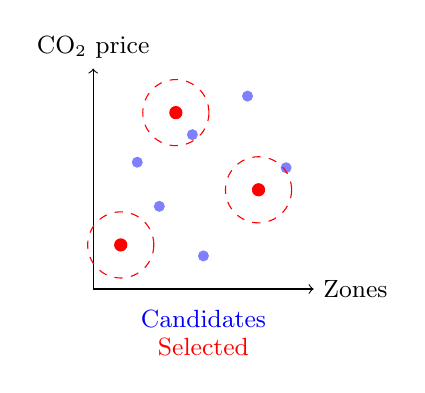
\begin{tikzpicture}[scale=0.7]
    % Parameter space
    \draw[->] (0,0) -- (4,0) node[right] {\small Zones};
    \draw[->] (0,0) -- (0,4) node[above] {\small CO$_2$ price};
    
    % Samples
    \foreach \x/\y in {0.5/0.8, 1.2/1.5, 2.0/0.6, 0.8/2.3, 3.0/1.8, 1.5/3.2, 2.8/3.5, 3.5/2.2, 1.8/2.8} {
        \fill[blue!50] (\x,\y) circle (0.1);
    }
    
    % Selected with coverage circles
    \fill[red] (0.5,0.8) circle (0.12);
    \draw[red,dashed] (0.5,0.8) circle (0.6);
    \fill[red] (3.0,1.8) circle (0.12);
    \draw[red,dashed] (3.0,1.8) circle (0.6);
    \fill[red] (1.5,3.2) circle (0.12);
    \draw[red,dashed] (1.5,3.2) circle (0.6);
    
    \node[align=center] at (2,-0.8) {\small \textcolor{blue}{Candidates}\\[-0.2em]\small \textcolor{red}{Selected}};
\end{tikzpicture}
\end{columns}
\end{frame}

\section{Stage 2: MILP Optimization}

\begin{frame}{MILP Formulation: Constraint Taxonomy}
\textbf{Zone-level Unit Commitment Model (Pyomo + HiGHS):}

\vspace{0.3em}
\begin{columns}
\column{0.5\textwidth}
\textbf{Generator Constraints:}
\begin{itemize}\setlength\itemsep{0em}
    \item Capacity: $p^{z,t} \leq P_{\max}^z \cdot u^{z,t}$
    \item Min generation: $p^{z,t} \geq P_{\min}^z \cdot u^{z,t}$
    \item Ramping: $|p^{z,t} - p^{z,t-1}| \leq R^z$
    \item Startup: $v^{z,t} \geq u^{z,t} - u^{z,t-1}$
\end{itemize}

\vspace{0.3em}
\textbf{Storage Constraints:}
\begin{itemize}\setlength\itemsep{0em}
    \item Power: $b_{\text{ch}}^{z,t}, b_{\text{dis}}^{z,t} \leq P_{\text{batt}}^z$
    \item SOC: {\small $\text{SOC}^{z,t} = \rho \cdot \text{SOC}^{z,t-1} + \eta \cdot b_{\text{ch}}^{z,t} - b_{\text{dis}}^{z,t}/\eta$}
    \item Final: $\text{SOC}_{\min}^z \leq \text{SOC}^{z,T} \leq \text{SOC}_{\max}^z$
\end{itemize}

\column{0.5\textwidth}
\textbf{Network Constraints:}
\begin{itemize}\setlength\itemsep{0em}
    \item Transmission: $|f^{\ell,t}| \leq F_{\ell}^{\max}$
    \item Power balance:
    {\small $\sum_{\text{gen}} = \text{demand} + \sum_{\text{storage}} + \sum_{\text{flows}}$}
\end{itemize}

\vspace{0.2em}
\textbf{Objective Function:}
\begin{align*}
\footnotesize
    \min \sum_{z,t} \Big[ &c_{\text{fuel}}^z \cdot p^{z,t} + C_{\text{start}}^z \cdot v^{z,t} + c_{\text{stor}}^z \cdot (b_{\text{ch}}^{z,t} + b_{\text{dis}}^{z,t}) \\
    &+ c_{\text{DR}}^z \cdot d_{\text{shed}}^{z,t} + c_{\text{VOLL}} \cdot u_{\text{unserv}}^{z,t} + c_{\text{spill}} \cdot s^{z,t} \Big]
\end{align*}
\end{columns}

\vspace{0.3em}
\begin{alertblock}{Complexity}
Typical scenario: \textbf{200K variables} (38K binary), \textbf{240K constraints}, solve time: \textbf{3--30 minutes}
\end{alertblock}
\end{frame}

\begin{frame}{Why MILP is Computationally Hard}
\begin{columns}
\column{0.5\textwidth}
\textbf{Binary Variable Explosion:}
\begin{itemize}
    \item Each thermal unit: 2 binaries/timestep
    \item 100 zones $\times$ 1.5 units $\times$ 96 timesteps $\times$ 2
    \item $\approx$ 29,000 binary variables
    \item Branch-and-bound tree: $2^{29000}$ worst-case nodes
\end{itemize}

\vspace{0.5em}
\textbf{Temporal Coupling:}
\begin{itemize}
    \item Ramping constraints link all timesteps
    \item Storage SOC creates Markov chains
    \item Prevents time decomposition
\end{itemize}

\column{0.5\textwidth}
\textbf{Spatial Coupling:}
\begin{itemize}
    \item Power balance couples all zones
    \item Transmission network creates dependencies
    \item Dense networks $\rightarrow$ harder to solve
\end{itemize}

\vspace{0.5em}
\textbf{Tight Feasibility Windows:}
\begin{itemize}
    \item Battery final SOC: $\pm 5$--18\% tolerance
    \item Minimum generation: 40\% of capacity
    \item Creates narrow feasible corridors
\end{itemize}
\end{columns}

\vspace{1em}
\begin{block}{Result}
2000 scenarios solved optimally. Median time: 8 minutes. 95th percentile: 45 minutes.
\end{block}
\end{frame}

\section{Stage 3: Graph Dataset Construction}

\begin{frame}{Heterogeneous Temporal Graph Representation}
\textbf{Key Insight:} Power systems are naturally multi-relational and temporal

\vspace{0.3em}
\begin{columns}
\column{0.5\textwidth}
\textbf{Hierarchical Node Types:}
\begin{itemize}\setlength\itemsep{-0.1em}
    \item \textcolor{darkblue}{Nation} (1 node)
    \item \textcolor{lightblue}{Regions} (2--13 nodes)
    \item \textcolor{cyan}{Zones} (50--150 nodes)
    \item \textcolor{gray}{Weather cells} (10--50 nodes)
\end{itemize}

\vspace{0.3em}
\textbf{Asset Node Types (per zone):}
\begin{itemize}\setlength\itemsep{-0.1em}
    \item \textcolor{orange}{Thermal} generators
    \item \textcolor{darkred}{Nuclear} units
    \item \textcolor{yellow}{Solar} farms
    \item \textcolor{lightblue}{Wind} farms
    \item \textcolor{blue}{Hydro reservoir} (controllable)
    \item \textcolor{blue!50}{Hydro run-of-river} (uncontrollable)
    \item \textcolor{green}{Battery} storage
    \item \textcolor{green!70!blue}{Pumped hydro} storage
    \item \textcolor{purple}{Demand Response}
\end{itemize}

\column{0.5\textwidth}
\textbf{Edge Types:}
\begin{itemize}\setlength\itemsep{-0.1em}
    \item Nation $\to$ Region (containment)
    \item Region $\to$ Zone (containment)
    \item Zone $\to$ Asset (ownership)
    \item Zone $\leftrightarrow$ Zone (transmission)
    \item Weather $\to$ Zone/Asset (influence)
    \item Asset $\to$ Asset (temporal: SOC, ramp, DR)
\end{itemize}

\vspace{0.3em}
\textbf{Node Features:}
\begin{itemize}\setlength\itemsep{-0.1em}
    \item \textbf{Static:} Capacity, costs, ramp rates, efficiency
    \item \textbf{Temporal (96 steps):} Demand, availability, dispatch, SOC
\end{itemize}

\vspace{0.3em}
\textbf{Graph Statistics:}
\begin{itemize}\setlength\itemsep{-0.1em}
    \item Total nodes: 100--800 (varies by scenario)
    \item Total edges: 200--2000
    \item Timesteps: 96 (15-min resolution)
\end{itemize}
\end{columns}

\end{frame}

\begin{frame}{Graph Construction Pipeline}
\begin{center}
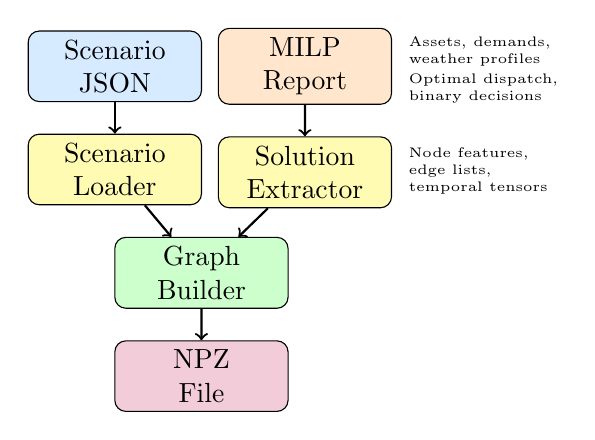
\begin{tikzpicture}[node distance=0.2cm,scale=0.95,
    box/.style={rectangle,draw,rounded corners,align=center,minimum width=2.2cm,minimum height=0.7cm}]
    
    \node[box,fill=lightblue!20] (json) {Scenario\\JSON};
    \node[box,fill=orange!20,right=of json] (report) {MILP\\Report};
    \node[box,fill=yellow!30,below=of json,yshift=-0.2cm] (loader) {Scenario\\Loader};
    \node[box,fill=yellow!30,below=of report,yshift=-0.2cm] (extractor) {Solution\\Extractor};
    \node[box,fill=green!20,below=of loader,xshift=1.1cm,yshift=-0.2cm] (builder) {Graph\\Builder};
    \node[box,fill=purple!20,below=of builder,yshift=-0.2cm] (npz) {NPZ\\File};
    
    \draw[->,thick] (json) -- (loader);
    \draw[->,thick] (report) -- (extractor);
    \draw[->,thick] (loader) -- (builder);
    \draw[->,thick] (extractor) -- (builder);
    \draw[->,thick] (builder) -- (npz);
    
    % Annotations
    \node[align=left,anchor=west,font=\tiny] at (3.8,0.2) {Assets, demands,\\weather profiles};
    \node[align=left,anchor=west,font=\tiny] at (3.8,-0.3) {Optimal dispatch,\\binary decisions};
    \node[align=left,anchor=west,font=\tiny] at (3.8,-1.4) {Node features,\\edge lists,\\temporal tensors};
\end{tikzpicture}
\end{center}

\vspace{0.5em}
\textbf{Key Design Decisions:}
\begin{itemize}\setlength\itemsep{0em}
    \item \textbf{Heterogeneous}: Different node/edge types preserve semantic meaning
    \item \textbf{Temporal}: Features stored as $[\text{nodes}, 96, \text{dim}]$ tensors
    \item \textbf{Hierarchical metadata}: Asset $\to$ Zone $\to$ Region mappings included
\end{itemize}
\end{frame}

\section{Stage 4: Hierarchical Encoder}

\begin{frame}{The Memory Problem with Dense Attention}
\begin{columns}
\column{0.5\textwidth}
\textbf{Naive Approach: HGT Transformer}
\begin{itemize}\setlength\itemsep{-0.1em}
    \item Heterogeneous Graph Transformer
    \item Dense attention: all nodes attend to all nodes
    \item Works for small graphs ($<$100 nodes)
\end{itemize}

\vspace{0.3em}
\textbf{Memory Requirement:}
\begin{equation*}
    \mathcal{O}(N^2 \cdot T \cdot H)
\end{equation*}
where:
\begin{itemize}\setlength\itemsep{-0.1em}
    \item $N \approx 600$ nodes
    \item $T = 96$ timesteps
    \item $H \approx 128$ hidden dim
\end{itemize}

\vspace{0.3em}
\textcolor{darkred}{\textbf{Result:} $>$40 GB GPU memory!}

\column{0.5\textwidth}
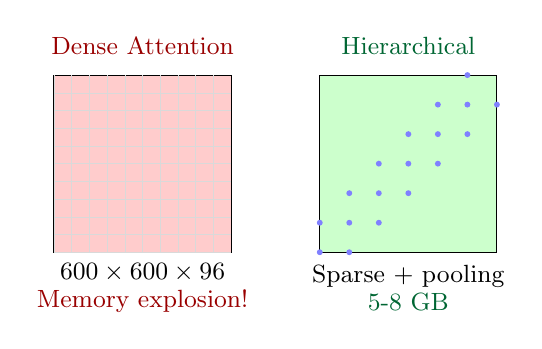
\begin{tikzpicture}[scale=0.75]
    % Dense attention matrix
    \draw[fill=red!20] (0,0) rectangle (3,3);
    \foreach \i in {0,0.3,...,3} {
        \draw[gray!30,very thin] (\i,0) -- (\i,3);
        \draw[gray!30,very thin] (0,\i) -- (3,\i);
    }
    \node at (1.5,3.5) {\small \textcolor{darkred}{Dense Attention}};
    \node[align=center] at (1.5,-0.6) {\small $600 \times 600 \times 96$\\[-0.2em]\small \textcolor{darkred}{Memory explosion!}};
    
    % Sparse alternative
    \begin{scope}[xshift=4.5cm]
        \draw[fill=green!20] (0,0) rectangle (3,3);
        % Sparse pattern
        \foreach \i in {0,0.5,...,2.5} {
            \fill[blue!50] (\i,\i) circle (0.05);
            \fill[blue!50] (\i+0.5,\i) circle (0.05);
            \fill[blue!50] (\i,\i+0.5) circle (0.05);
        }
        \node at (1.5,3.5) {\small \textcolor{darkgreen}{Hierarchical}};
        \node[align=center] at (1.5,-0.6) {\small Sparse + pooling\\[-0.2em]\small \textcolor{darkgreen}{5-8 GB}};
    \end{scope}
\end{tikzpicture}
\end{columns}

\vspace{0.5em}
\begin{alertblock}{Solution}
\textbf{Hierarchical pooling} with sparse attention at each level
\end{alertblock}
\end{frame}

\begin{frame}{Hierarchical Temporal Encoder Architecture}
\begin{center}
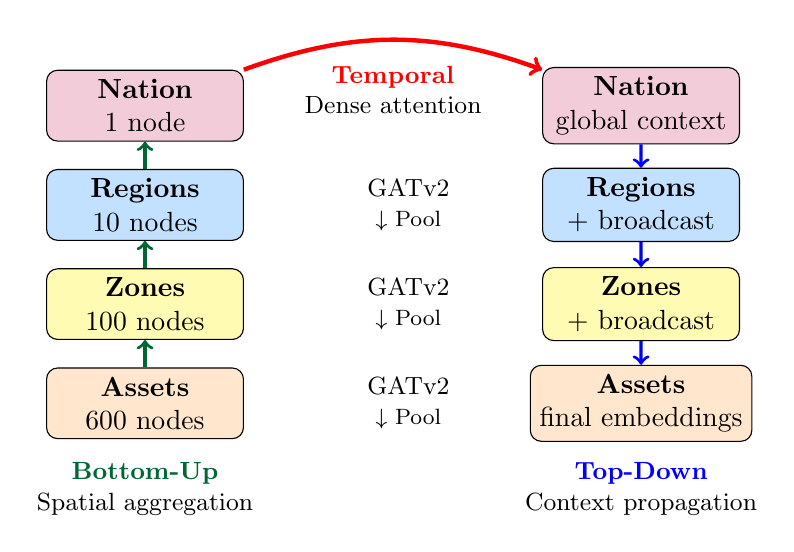
\begin{tikzpicture}[scale=0.9,
    level/.style={rectangle,draw,rounded corners,align=center,minimum width=2.5cm,minimum height=0.7cm}]
    
    % Bottom-up encoding
    \node[level,fill=orange!20] at (0,0) (assets) {\textbf{Assets}\\600 nodes};
    \node[level,fill=yellow!30] at (0,1.4) (zones) {\textbf{Zones}\\100 nodes};
    \node[level,fill=lightblue!30] at (0,2.8) (regions) {\textbf{Regions}\\10 nodes};
    \node[level,fill=purple!20] at (0,4.2) (nation) {\textbf{Nation}\\1 node};
    
    % Operations
    \node[align=center,font=\small,anchor=west] at (3,0) {GATv2\\{\footnotesize $\downarrow$ Pool}};
    \node[align=center,font=\small,anchor=west] at (3,1.4) {GATv2\\{\footnotesize $\downarrow$ Pool}};
    \node[align=center,font=\small,anchor=west] at (3,2.8) {GATv2\\{\footnotesize $\downarrow$ Pool}};
    
    % Arrows up
    \draw[->,very thick,darkgreen] (assets) -- (zones);
    \draw[->,very thick,darkgreen] (zones) -- (regions);
    \draw[->,very thick,darkgreen] (regions) -- (nation);
    
    % Top-down propagation
    \node[level,fill=purple!20] at (7,4.2) (nation2) {\textbf{Nation}\\global context};
    \node[level,fill=lightblue!30] at (7,2.8) (regions2) {\textbf{Regions}\\+ broadcast};
    \node[level,fill=yellow!30] at (7,1.4) (zones2) {\textbf{Zones}\\+ broadcast};
    \node[level,fill=orange!20] at (7,0) (assets2) {\textbf{Assets}\\final embeddings};
    
    \draw[->,very thick,blue] (nation2) -- (regions2);
    \draw[->,very thick,blue] (regions2) -- (zones2);
    \draw[->,very thick,blue] (zones2) -- (assets2);
    
    % Connection
    \draw[->,ultra thick,red] (nation) to[bend left=20] (nation2);
    
    % Labels
    \node[align=center,anchor=north,font=\small] at (0,-0.7) {\textcolor{darkgreen}{\textbf{Bottom-Up}}\\Spatial aggregation};
    \node[align=center,anchor=north,font=\small] at (3.5,4.9) {\textcolor{red}{\textbf{Temporal}}\\Dense attention};
    \node[align=center,anchor=north,font=\small] at (7,-0.7) {\textcolor{blue}{\textbf{Top-Down}}\\Context propagation};
\end{tikzpicture}
\end{center}

\vspace{0.2em}
\textbf{Key Innovation:} Sparse spatial aggregation + dense temporal modeling at top level only
\end{frame}

\begin{frame}{Training Configuration \& Results}
\begin{columns}
\column{0.5\textwidth}
\textbf{Model Hyperparameters:}
\begin{itemize}\setlength\itemsep{-0.1em}
    \item Hidden dim: 128
    \item Spatial layers: 2 per level
    \item Temporal layers: 4 (Transformer)
    \item Attention heads: 8
    \item Dropout: 0.1
\end{itemize}

\vspace{0.3em}
\textbf{Training Setup:}
\begin{itemize}\setlength\itemsep{-0.1em}
    \item Dataset: 2000 graphs
    \item Split: 70\% train, 15\% val, 15\% test
    \item Batch size: 1 (full graph)
    \item Optimizer: AdamW ($lr = 3 \times 10^{-4}$)
    \item Epochs: 150
    \item Loss: Contrastive (multi-scale)
\end{itemize}

\column{0.5\textwidth}
\textbf{Memory Efficiency:}
\begin{itemize}\setlength\itemsep{-0.1em}
    \item Assets GAT: $\sim$2 GB
    \item Zones GAT: $\sim$300 MB
    \item Regions GAT: $\sim$20 MB
    \item Transformer: $\sim$100 MB
    \item \textbf{Total: $\sim$5 GB} (\textcolor{darkgreen}{8$\times$ reduction!})
\end{itemize}

\vspace{0.3em}
\textbf{Training Performance:}
\begin{itemize}\setlength\itemsep{-0.1em}
    \item Time per epoch: $\sim$12 minutes (A100)
    \item Convergence: $\sim$100 epochs
    \item Current loss: $\sim$3 (\textcolor{darkgreen}{75\% less than initial})
\end{itemize}
\end{columns}

\vspace{0.5em}
\begin{block}{Status}
\textcolor{darkgreen}{\textbf{Training completed.}} Multi-scale embeddings generated for all 2000 scenarios.
\end{block}
\end{frame}

\begin{frame}{Generated Embeddings: Multi-Scale Representation}
\textbf{Output Structure:}

\vspace{0.5em}
\begin{center}
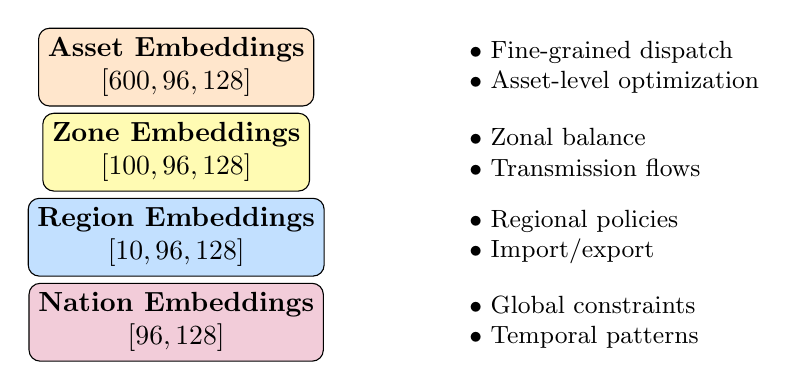
\begin{tikzpicture}[scale=0.9,
    box/.style={rectangle,draw,rounded corners,align=center,minimum width=3cm,minimum height=0.8cm}]
    
    \node[box,fill=orange!20] at (0,0) (assets) {\textbf{Asset Embeddings}\\$[600, 96, 128]$};
    \node[box,fill=yellow!30] at (0,-1.2) (zones) {\textbf{Zone Embeddings}\\$[100, 96, 128]$};
    \node[box,fill=lightblue!30] at (0,-2.4) (regions) {\textbf{Region Embeddings}\\$[10, 96, 128]$};
    \node[box,fill=purple!20] at (0,-3.6) (nation) {\textbf{Nation Embeddings}\\$[96, 128]$};
    
    % Use cases
    \node[align=left,anchor=west,font=\small] at (4,0) {$\bullet$ Fine-grained dispatch\\$\bullet$ Asset-level optimization};
    \node[align=left,anchor=west,font=\small] at (4,-1.2) {$\bullet$ Zonal balance\\$\bullet$ Transmission flows};
    \node[align=left,anchor=west,font=\small] at (4,-2.4) {$\bullet$ Regional policies\\$\bullet$ Import/export};
    \node[align=left,anchor=west,font=\small] at (4,-3.6) {$\bullet$ Global constraints\\$\bullet$ Temporal patterns};
\end{tikzpicture}
\end{center}

\vspace{0.5em}
\textbf{What do embeddings capture?}
\begin{itemize}
    \item \textbf{Local:} Asset-specific operational constraints (ramp rates, min/max power)
    \item \textbf{Mesoscale:} Zonal interactions (transmission bottlenecks, local imbalances)
    \item \textbf{Global:} System-wide patterns (peak demand periods, renewable variability)
\end{itemize}
\end{frame}

\section{Next Steps: Energy-Based Model}

\begin{frame}{Next Step: Energy-Based Model}
\textbf{Goal:} Learn to sample feasible, near-optimal UC configurations

\vspace{0.3em}
\begin{columns}
\column{0.48\textwidth}
\textbf{Ising-EBM Framework:}
\begin{equation*}
    E(u | h) = -\sum_i h_i u_i - \sum_{i<j} J_{ij} u_i u_j
\end{equation*}
where:
\begin{itemize}\setlength\itemsep{-0.1em}
    \item $u_i \in \{0,1\}$: Binary commitment
    \item $h_i$: Local fields (from embeddings)
    \item $J_{ij}$: Coupling weights
    \item $E$: Energy (lower = better)
\end{itemize}

\vspace{0.3em}

\column{0.48\textwidth}
\textbf{Gibbs Sampling:}
\begin{equation*}
    P(u_i=1 | u_{-i}) = \frac{1}{1 + \exp\left(-\frac{2\Delta E_i}{T}\right)}
\end{equation*}
{\footnotesize Sequential single-spin flips at temperature $T$}

\vspace{0.3em}
\textbf{Training:}
\begin{itemize}\setlength\itemsep{-0.1em}
    \item Contrastive divergence
    \item Supervised: match MILP solutions
    \item Learn $h_i$ and $J_{ij}$ from embeddings
\end{itemize}

\column{0.48\textwidth}
\begin{center}
\begin{tikzpicture}[node distance=1.2cm, scale=1.0,
    box/.style={rectangle,draw,rounded corners,align=center,minimum width=2.8cm,minimum height=0.75cm}]
    
    \node[box,fill=orange!20] at (0,3.6) (embed) {\textbf{Embeddings}\\{\small Multi-scale $h$}};
    \node[box,fill=yellow!30] at (0,2.2) (config) {\textbf{UC Config}\\{\small Binary $u_i$}};
    \node[box,fill=lightblue!30] at (0,0.8) (ising) {\textbf{Ising Model}\\{\small $E(u|h)$}};
    \node[box,fill=green!20] at (0,-0.6) (gibbs) {\textbf{Gibbs Sampler}\\{\small Sequential flips}};
    
    \draw[->,very thick] (embed) -- (ising);
    \draw[->,very thick] (config) -- (ising);
    \draw[->,very thick,red] (ising) -- (gibbs);
    
    \node[align=center,anchor=north,font=\small] at (0,-1.5) {\textcolor{darkgreen}{Sample diverse\\feasible solutions}};
\end{tikzpicture}
\end{center}
\end{columns}

\vspace{0.3em}
\begin{alertblock}{Status}
Next milestone: EBM architecture design \& training
\end{alertblock}
\end{frame}


\section{Results \& Validation}

\begin{frame}{Current Achievements}
\begin{columns}
\column{0.5\textwidth}
\textbf{Dataset:}
\begin{itemize}
    \item \textcolor{darkgreen}{\checkmark} 2000 diverse scenarios
    \item \textcolor{darkgreen}{\checkmark} All solved to optimality (MILP)
    \item \textcolor{darkgreen}{\checkmark} 2000 heterogeneous temporal graphs
    \item \textcolor{darkgreen}{\checkmark} Average solve time: 8 minutes
\end{itemize}

\vspace{0.5em}
\textbf{Encoder:}
\begin{itemize}
    \item \textcolor{darkgreen}{\checkmark} Hierarchical architecture implemented
    \item \textcolor{darkgreen}{\checkmark} Training completed (100 epochs)
    \item \textcolor{darkgreen}{\checkmark} Multi-scale embeddings generated
    \item \textcolor{darkgreen}{\checkmark} Memory: 5 GB (vs 40+ GB naive)
\end{itemize}

\column{0.5\textwidth}
\textbf{Validation Metrics:}
\begin{itemize}
    \item Embedding quality: Good convergence
    \item Contrastive loss: 3.6
    \item Representation learning successful
\end{itemize}

\vspace{0.5em}
\textbf{Next Milestones:}
\begin{enumerate}
    \item Design \& train Ising-EBM architecture
    \item Implement Gibbs sampler for thermodynamic sampling
    \item Implement LP worker for continuous dispatch
    \item Integrate hybrid pipeline: Encoder → EBM → Gibbs → LP
    \item Benchmark: Hybrid vs pure MILP
    \item Measure:
    \begin{itemize}
        \item Speed-up factor
        \item Optimality gap
        \item Feasibility rate
    \end{itemize}
\end{enumerate}
\end{columns}

\vspace{1em}
\begin{block}{Timeline}
EBM integration: 2--3 weeks. Full validation: 4--6 weeks.
\end{block}
\end{frame}

\begin{frame}{Technical Contributions}
\begin{enumerate}
    \item \textbf{Benchmark Dataset:}
    \begin{itemize}
        \item First large-scale UC benchmark with hierarchical structure
        \item 2000 diverse, realistic scenarios
        \item Ground truth optimal solutions from MILP
    \end{itemize}
    
    \item \textbf{Hierarchical GNN Architecture:}
    \begin{itemize}
        \item Scalable to 600+ nodes $\times$ 96 timesteps
        \item 8$\times$ memory reduction vs dense attention
        \item Multi-scale embeddings for coarse-to-fine reasoning
    \end{itemize}
    
    \item \textbf{Heterogeneous Temporal Graphs:}
    \begin{itemize}
        \item Preserves semantic structure of power systems
        \item Multiple node/edge types
        \item Temporal features + static metadata
    \end{itemize}
    
    \item \textbf{Hybrid Optimization Framework (in progress):}
    \begin{itemize}
        \item Combines learning (GNN, EBM) with optimization (LP, MILP)
        \item Fast sampling + feasibility guarantees
        \item Warm-starting for hard instances
    \end{itemize}
\end{enumerate}
\end{frame}

\section{Conclusion}

\begin{frame}{Summary}
\textbf{Problem:} Unit commitment at asset level is computationally intractable

\vspace{0.5em}
\textbf{Our Approach:}
\begin{enumerate}
    \item Generate diverse synthetic scenarios with MILP-solvable complexity
    \item Solve at zone level to get ground truth optimal solutions
    \item Build hierarchical graph dataset preserving multi-scale structure
    \item Train scalable hierarchical encoder with sparse attention
    \item \textit{(Next)} Use embeddings to guide EBM sampling at asset level
\end{enumerate}

\vspace{0.5em}
\textbf{Current Status:}
\begin{itemize}
    \item \textcolor{darkgreen}{\textbf{Completed:}} Stages 1--4 (data generation, MILP solving, graph construction, encoder training)
    \item \textcolor{orange}{\textbf{In Progress:}} Stage 5 (EBM integration)
    \item \textcolor{blue}{\textbf{Next:}} Validation \& benchmarking
\end{itemize}

\vspace{0.5em}
\textbf{Expected Impact:}
\begin{itemize}
    \item $10$--$100\times$ speed-up for large-scale UC problems
    \item Enable real-time asset-level optimization
    \item Transferable to other combinatorial optimization domains
\end{itemize}
\end{frame}

\begin{frame}{Open Questions \& Future Work}
\begin{columns}
\column{0.5\textwidth}
\textbf{Methodological:}
\begin{itemize}
    \item EBM vs direct regression: trade-offs?
    \item Optimal sampling temperature schedule?
    \item How to handle infeasible samples?
    \item LP projection vs MILP warm-start?
\end{itemize}

\vspace{0.5em}
\textbf{Scalability:}
\begin{itemize}
    \item Extend to multi-day horizons?
    \item Online learning from new scenarios?
    \item Transfer to real power systems?
\end{itemize}

\column{0.5\textwidth}
\textbf{Extensions:}
\begin{itemize}
    \item Stochastic UC (uncertainty in demand/renewables)
    \item Security-constrained UC (N-1 contingencies)
    \item Multi-objective optimization (cost vs emissions)
    \item Integration with market mechanisms
\end{itemize}

\vspace{0.5em}
\textbf{Validation:}
\begin{itemize}
    \item Compare with state-of-the-art UC heuristics
    \item Benchmark on real utility datasets
    \item Sensitivity analysis on architecture choices
\end{itemize}
\end{columns}
\end{frame}



% Backup slides
\appendix

\begin{frame}{Backup: Scenario Statistics}
\textbf{Generated Scenario Characteristics:}

\vspace{0.5em}
\begin{table}
\centering
\begin{tabular}{lrrr}
\toprule
\textbf{Metric} & \textbf{Min} & \textbf{Median} & \textbf{Max} \\
\midrule
Regions & 2 & 7 & 13 \\
Zones & 4 & 87 & 140 \\
Thermal units & 0 & 120 & 315 \\
Solar/Wind farms & 50 & 180 & 350 \\
Binary variables & 0 & 23,040 & 60,480 \\
Continuous variables & 8,640 & 168,000 & 268,800 \\
Constraints & 12,000 & 185,000 & 302,000 \\
MILP solve time (sec) & 45 & 480 & 2700 \\
\bottomrule
\end{tabular}
\end{table}

\vspace{0.5em}
\textbf{Diversity Metrics:}
\begin{itemize}
    \item Coverage of parameter space: 87\%
    \item Minimum pairwise distance: 0.35 (normalized)
    \item Weather profiles: All 5 types represented
    \item CO$_2$ price range: Full spectrum covered
\end{itemize}
\end{frame}


\end{document}
